\section{Hypothesentests}
\subsection{PE-File Korrumpierung bei mehrstufiger Obfuskierung}
Das Experiment hat gezeigt, dass insgesamt 23,4\% der vorhandenen Samples korrumpiert waren. Von den mehrstufigen Obfuskationen waren 0.7\% korrumpiert. Der Anteil an Korrumpierung unter den mehrstufigen Obfuskationen lag bei 1,4\%.  Allerdings zeigt sich in Tabelle \ref{tab:corrupted_files}, dass die meisten Korruptionen bei Windows Defender aufgetreten sind und unter MDE fast keine. Insgesamt sind die mehrstufigen Korruptionen deutlich seltener gewesen als die einstufigen korrupten Files. Dies kann ein Ergebnis des genetischen Algorithmus sein, der die Lösungen Teil für Teil konstruiert und so viele fehlerhafte einstufige Teile hat, bevor er die erfolgreichen mit anderen Kandidaten rekombiniert. 
In keinem der Fälle wurde das Niveau von 25\% überschritten, was dafür spricht, dass ein Großteil der dargebotenen Files eine sehr solide Rate von Ausführbarkeit beweist und der Algorithmus nicht langwierig in unausführbaren Stacks herumsucht. Gegenüberstellung der Korrumpierungsanteile von allen Dateien gegen die mehrstufigen Dateien findet sich in Abbildung \ref{fig:corrupt_vs_multi}.

\begin{figure}[h]
    \centering
    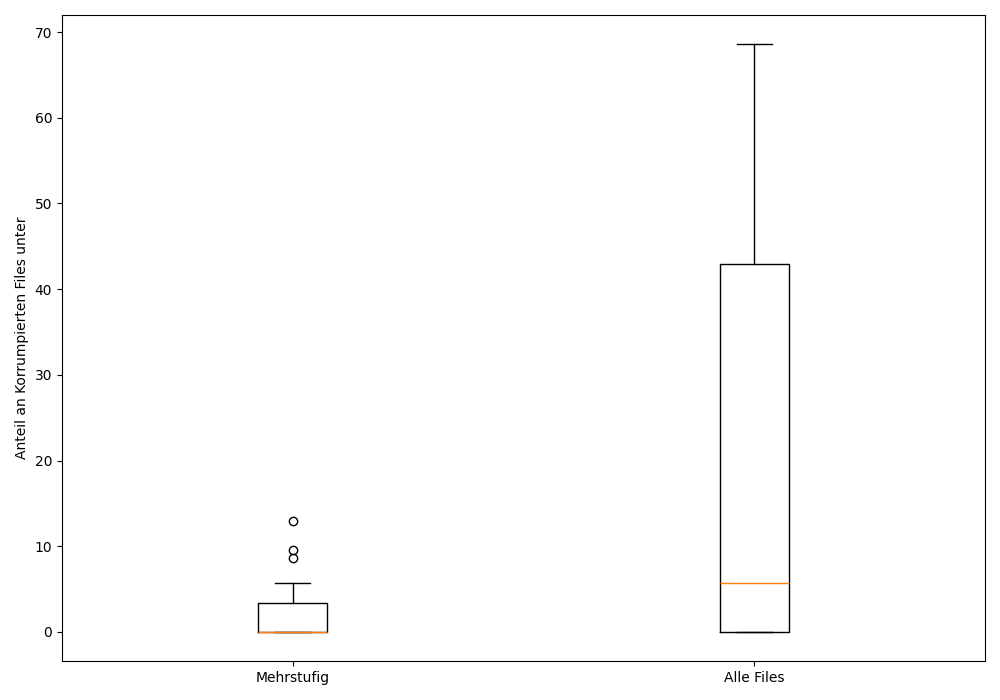
\includegraphics[width=0.85\textwidth]{gfx/Hypothesendiagramme/corruption_vs_multi_corruption.png}
    \caption{Anteil der Korrumpierten Dateien}
    \label{fig:corrupt_vs_multi}
\end{figure}

\subsubsection{Testauswahl}
Aufgrund der geringen Stichprobe von \textit{N = 18} wurde sich gegen einen Z Test und für einen Binomialtest anhand der Anteile von Korruption entschieden, der wie in Codebeispiel \ref{Code:Corruption_test} durchgeführt wurde.

\begin{listing}
    \begin{minted}{Python}
corrupted_multiparts_over_number_multiparts= 
    [0.0, 0.0, 0.0, 0.0,  0.0, 0.0,
    0.04545, 0.06667, 0.0, 0.0, 0.0, 0.03,
    0.0,  0.05, 0.0, 0.0, 0.0, 0.0]
print(np.mean(corrupted_multiparts_over_number_multiparts))
print(percentage_corrupt_of_multiparts)
n = len(percentage_corrupt_of_multiparts)
k = sum(1 for p in percentage_corrupt_of_multiparts if p >0.25)
p_value_binom= binomtest(k,n, p =0.25, alternative='greater')
print(p_value_binom)
    \end{minted}
    \label{Code:Corruption_test}
    \caption{Hypothesentest Korrumpierte mehrstufige}
\end{listing}

\subsubsection{Ergebnis}
Der Test hat einen mittleren Korrumpierungsanteil von 1,06\% ergeben. Der P-Test (\textbf{p = 1.0} hat die Nullhypothese von einem Anteil von kleiner-gleich 25\% beibehalten und die Hypothese somit wiederlegt.

\subsubsection{Explorative Untersuchung}
Der gleiche Test wurde mit dem Anteil aller korrumpierten Files an allen erstellten Files wiederholt und ergab dabei einen Mittelwert von 23,4\% und einen p-Wert von 0.019. Hierbei lässt sich also schon deutlich eher eine Tendenz von mehr als 25\% korrumpierter Dateien vermuten, aber auch bei einem Signifikanzniveau von 1\% lässt sich diese Hypothese nicht nachweisen.

% subsection{Geringe Shellcode Korrumpierung}
% Todo bei neuem Experiment
% 
%\textbf{Eventuelle Streichung bei keiner Verbesserung des Ergebnisses}

\subsection{Red-Teaming Kriterien Erfüllung}
Aus dem Experiment hat sich - abgesehen von den architektonischen Details - gezeigt, dass die zwei wesentlichen Anforderungen für den praktischen Einsatz mit den gestellten Konfigurationen erfüllt werden können.
So hat sich nicht nur gezeigt, dass die Laufzeit aller Experimente (Tabelle \ref{tab:runtime}) unterhalb der Zeit lag, die maximal verwendet werden darf, sondern auch gezeigt, dass in jedem Experiment mindestens eine erfolgreiche Evasion Lösung erstellt werden konnte\footnote{Eine Wiederholung des Algorithmus war nötig, aber die zusätzliche Zeit wurde mit einberechnet}, die von einem AV Scanner nicht erkannt wurde. Auch könnte man die Laufzeit des Algorithmus noch weiter optimieren, indem der Algorithmus sofort beim finden einer einzelnen Lösung terminiert und somit potentiell weitere Zeit erspart. Für die Fragestellung war dies jedoch nicht zielführend, weswegen dieses Feature hier nicht implementiert worden ist.

\subsubsection{Testauswahl}
Da die Einschätzung über die Verwendbarkeit des Tools für Red Teaming nicht mithilfe eines statistischen Tests bestimmt werden kann, müssen andere Kriterien hierfür herangezogen werden. In \ref{Methode:Kriterien} wurden diese bereits genannt. Hierbei handelt es sich um die Erfolgsaussichten (Wie wahrscheinlich bekomme ich ein Ergebnis mit den gewünschten Eigenschaften?), der Laufzeit (Wie lange brauche ich, um bis zum gewünschten Ergebnis zu kommen?) und Ressourcenverbrach (Welche Kosten und welche Arbeitszeit erzeugt die Nutzung des Tools?).
\paragraph{Erfolgswahrscheinlichkeit}
Die \textit{Erfolgsaussichten} sollen naturgemäß möglich hoch sein und können nicht höher als 100\% werden. Um einen belastbaren Vergleich zu schaffen wird ein Fehlerniveau von 5\% akzeptiert und eine Erfolgsrate von 95\% angesetzt. Hierbei wird ein Erfolg damit erklärt, dass in einem Durchlauf ein erfolgreiches Ergebnis generiert wird. 
\paragraph{Laufzeit}
Als bisherige Angabe für die \textit{Laufzeit} wurde bisher ein Wert von 2 Stunden also 7200 Sekunden angepeilt. Hinsichtlich der Ergebnisse aus Abbildung \ref{fig:runtime_overview} lässt sich schon sehr deutlich erkennen, dass diese eingehalten wird. Aus diesem Grund soll das ambitioniertere Ziel von 10 Minuten = 600 Sekunden für den Vergleich mit den Daten herhalten.
Die Laufzeitprüfung wird mit einem T-Test durchgeführt, da die Laufzeitdaten Normalverteilt sind und kontinuierliche Daten sind.
\begin{listing}
    \begin{minted}{Python}
laufzeiten = [436, 478, 530, 377, 493, 454, 
410, 392, 496, 493, 468, 488,
375, 402, 389, 372, 818, 413]
laufzeit_zielwert = 600
t_stat, p_value = ttest_1samp(laufzeiten, laufzeit_zielwert, alternative='less')
print(f"T-Statistik: {t_stat}")
print(f"p-Wert: {p_value}")
    \end{minted}
    \caption{einseitiger T-Test auf Laufzeit}
    \label{listing:Laufzeittest}
\end{listing}
\paragraph{Resourcenverbrauch}
Hinsichtlich des \textit{Resourcenverbrauchs} lassen sich zwei Bestandteile feststellen. Einmal die laufenden Kosten für die Infrastruktur, auf welcher die Tools laufen und ausgeführt werden, sowie die Arbeitszeit, die zum Konfigurieren, Hochfahren und Starten des Tools nötig ist. Für ersteres kann die Laufzeit einfach mit den Kosten für die Infrastruktur multipliziert werden.
Zweiteres ist schwieriger zu quantifizieren, ohne ein eigenständiges Experiment zum Userverhalten und Arbeitsgeschwindigkeit durchzuführen. Aus diesem Grund wird ein Vergleich zum Basistool (Obscurus) gezogen, auch um argumentieren zu können, inwiefern die (zusätzlichen) Kosten sich mit dem Ergebnis begründen lassen.
\subsubsection{Testergebnis}
Der T-Test für die \textit{Laufzeit} ergab einen P-Wert von 0.000011 und damit zu einem sigfinikanten Ergebnis. Dies bedeutet, dass die Laufzeit des Tools (im Mittel) weniger als 10 Minuten beträgt.
Der Binomialtest für die \textit{Erfolgsaussichten} des Tools ergab einen P-Wert von 0.77 und damit zu keinem signifikanten Ergebnis. Dies bedeutet, dass nicht davon ausgegangen werden kann, dass das Tool in mehr als 95\% der Fälle im ersten Durchlauf zu einem Ergebnis kommt.
Der Ressourcenverbrauch verteilt sich auf mehrere Komponenten. Obscurus und Obscurus Evolution benötigen beide die Instanzen der Obfuskatoren und AV Scanner (2 Obfuskatoren, 1 AV Scanner). Obscurus benötigt weiterhin einen Webserver, wohingegen Obscurus Evolution die Ausführungsumgebung für den genetischen Algorithmus benötigt. Man kann argumentieren, dass sowohl der Webserver als auch der genetische Algorithmus auf einer der Obfuskatorinstanzen laufen können, da sie selbst nicht viel Rechenleistung benötigen. Hier ergibt sich dadurch aber ein Gleichstand in den verwendeten Instanzen.
Obscurus ist als Tool mit seiner Einmalausführung deutlich schneller als Obscurus Evolution und benötigt im Mittel etwa 30 Sekunden für einen Durchlauf (N=5). ObscurusEvolution benötigt weniger als 600 Sekunden für einen vollständigen Durchlauf (s.o.). Damit sind die Kosten von Obscurus Evolution in diesem Teil etwa 5 Mal so hoch, wie die von Obscurus Evolution.
Zur Einrichtung von Obscurus Evolution benötigt man die gleichen Voraussetzungen, wie sie für Obscurus selbst, ohne dass man den Webserver prüfen und die statistische Analyse für die Heuristik laufen lassen muss, welche im Zentrum vom automatischen Modus von Obscurus steht. Stattdessen kann bei Obscurus Evolution jedoch noch die Mutations-, Rekombinationschance, das Rekombinations- und Mutationsverhalten und die Initalpopulation konfiguriert wird. In diesem Bereich brauchen beide Tools Arbeitszeit.
Aus diesen Betrachtungen ergibt sich, dass Obscurus Evolution deutlich mehr Zeit als der Vorgänger benötigt und damit zwischen 2 und 5 Mal so teuer ist, was den Ressourcenverbrauch betrifft. Die monetären Kosten betragen pro Stunde etwa 5 Cent, was mit großzügiger Verwendung von einzelnen Instanzen für alles und der Verwendung von beiden AV-Scannern gleichzeitig (5 Instanzen) auf 25 Cent/Stunde beläuft. Die tatsächlichen Gesamtkosten pro Durchlauf betragen somit etwa $25ct/Stunde\times 10 Minuten = 4 Cent$. Und können als vernachlässigbar angesehen werden.


Aus diesen zusammengetragenen Ergebnissen lässt sich schließen, dass Obscurus Evolution zwar eine Weiterentwicklung von Obscurus ist, die die Kriterien an Ressourcenverbrauch und Laufzeit einhält, allerdings keine nachweisliche Erhöhung der Erfolgsaussichten im ersten Durchlauf bewirken kann.

\subsubsection{Weitere Betrachtung}
Betrachtet man den Aufbau des Tools, so stellt man fest, dass einige Optimierungen für den produktiven Einsatz möglich sind. So könnte man den genetischen Algorithmus bereits dann terminieren lassen, sobald eine einzelne Lösung gefunden wurde und solange weiterlaufen lassen, bis dies geschieht und nicht nur die demonstrierten 20 Generationen. Im Experiment ist es nur einmal vorgekommen, dass keine Lösung im ersten Versuch gefunden wurde; als dieses Problem dann erneut bearbeitet wurde, hat der Algorithmus 4 Lösungen gefunden. Aus diesen Einschränkungen lässt sich argumentieren, dass das Tool auf ähnlich hohem Niveau wie Obscurus selbst arbeitet und zumindest die Mehrkosten wett macht.


\subsection{Einfluss der Länge von Obfuskatorkaskaden}

 \subsubsection{Testauswahl}
 Da es für diesen Test zwei unabhängige Variablen (AV Scanner und Malware Typ) und nur eine abhängige Variable (Anzahl der Obfuskationsschritten von Erfolgreichen Kandidaten) gibt, wird hier eine zweifaktorielle ANOVA durchgeführt.

\begin{listing}
    \begin{minted}{Python}
import statsmodels.api as sm
import pandas as pd
from statsmodels.formula.api import ols

data ={
    'Malware_Type': ['Benign']*24 + ['Calc']*24 + ['Shell']*15,
    'AV_Scanner': ['MDE']*10 + ['WD']*14 + 
        ['MDE'] *15 + ['WD'] *9 + 
        ['MDE']*11 + ['WD']*4,
    'Steps':  [1]*8+[2]*2+[1]*9+[2]*4+[4] + 
        [1]*5 + [2]*10 + [1]*5 + [2]*4+ 
        [2]*9 + [3]*2 + [2]*4
} 

df = pd.DataFrame(data)
model = ols('Steps ~ C(Malware_Type) * C(AV_Scanner)', data=df).fit()
anova_table = sm.stats.anova_lm(model, typ=2)

print(anova_table)
    \end{minted}
\end{listing}

 \subsubsection{Testergebnis}
 In Tabelle \ref{tab:ANOVA} sieht man die Ergebnisse der multifaktoriellen ANOVA. Es stellt sich heraus, dass der Malware Typ als einziges einen signfikanten Unterschied in den nötigen Schritten bewirkt und weder der AV-Scanner noch das AV-Scanner - Malware Typ Paar signifikant zur Varianzaufklärung beitragen.
\begin{table}[hp]
\begin{tabular}{@{}lllll@{}}
\toprule
                           & sum\_sq   & df   & F        & PR(\textgreater{}F) \\ \midrule
Malware Typ                & 5.113966  & 2.0  & 7.967892 & \textit{0.000888}            \\
AV Scanner                 & 0.000077  & 1.0  & 0.000241 & 0.987679            \\
Malware Typ und AV Scanner & 0.899670  & 2.0  & 1.401745 & 0.254523            \\
Residual                   & 18.291919 & 57.0 & NaN      & NaN                 \\ \bottomrule
\end{tabular}
\caption{ANOVA Ergebnis Obfuskationsschritte}
\label{tab:ANOVA}
\end{table} 
\begin{figure}[h]
    \centering
    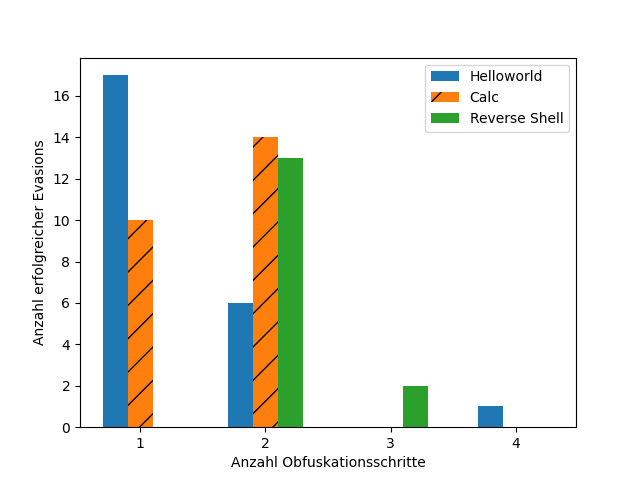
\includegraphics[width=0.85\textwidth]{gfx/Hypothesendiagramme/combined_obfuscation_steps.png}
    \caption{Anzahl der Obfuskationschritte bei erfolgreichen Kandidaten in Abhängigkeit vom Malwaretyp}
    \label{fig:steps_per_Solve}
\end{figure}

\subsubsection{weitere Betrachtung}
Wie bereit ins \ref{fig:steps_per_Solve} absehbar, zeichnet sich ein Trend ab, was die nötigen Obfuskationsschritte pro Malwaretyp angeht. So scheint es, dass Shell Access Malware längerstufige Obfuskationsschritte benötigt, als die anderen beiden getesteten Files. Für die Benign-Testcases hat sich weiterhin gezeigt, dass am häufigsten eine kurze Lösung zum Erfolg führte, aber auch eine (unnötig) lange Lösung mit 4 Schritten dem Scanner entgehen konnte. Ein möglicher Schluss lautet, dass die Freiheitsgrade, die zur Evasion zur Verfügung stehen, geringer werden, je interaktiver Malware ist. Dies würde zumindest erklären, warum bei dem Benigntestcase auch Lösungen mit 4 Schritten erfolgreich waren.

\begin{table}[h]
    \centering
    \begin{tabular}{|p{0.3\textwidth}|l|l|}
        \hline
        \textbf{Hypothese} & \textbf{Ergebnis} & \textbf{Indizien} \\ \hline
        Hypothese 1: PE Korrumpierung steigt mit mehreren Obfuskationen & Widerlegt& Binomialtest + Abbildung \ref{fig:corrupt_vs_multi} \\ \hline
        Hypothese 2: Red Teaming Kriterien erfüllbar & Bestätigt & Argumentation \\ \hline
        Hypothese 3: Zusammenhang von Malware Typ und Obfuskation & Bestätigt & ANOVA Tab. \ref{tab:ANOVA} \\ \hline
    \end{tabular}
    \caption{Übersicht über die Hypothesenprüfung des Papers}
    \label{tab:hypothesenpruefung}
\end{table}